\documentclass{beamer}
\usepackage[utf8]{inputenc}
\usepackage{subfig}
\usepackage{utopia} %font utopia imported
\usepackage{arabtex}
\usepackage{utf8}
\setcode{utf8}
\usetheme{Madrid}
\usecolortheme{default}

% This block of code defines the information to appear in the
% title page

\title[Crosstalk ] %optional
{Signal Integrity and Crosstalk effect}

\subtitle{Errors Can Break Your ASIC!}

\author[Ahmed Abdelazeem] % (optional)
{Ahmed Abdelazeem}
%{A.~B.~Arthur\inst{1} \and J.~Doe\inst{2}}

\institute[ZU] % (optional)
{
	Faculty of Engineering\\
	Zagazig University
}
%{
	%	\inst{1}%
	%	Faculty of Engineering\\
	%	Zagazig University
	%	\and
	%	\inst{2}%
	%	Faculty of Chemistry\\
	%	Very Famous University
	%}

\date[ZU 2023] % (optional)
{RTL2GDSII Flow, February 2022}

%\logo{
\includegraphics[height=1.5cm]{lion-logo.png}}

%End of title page configuration block
%------------------------------------------------------------

%------------------------------------------------------------
%The next block of commands puts the table of contents at the
%beginning of each section and highlights the current section:

\AtBeginSection[]
{
	\begin{frame}
		\frametitle{Table of Contents}
		\tableofcontents[currentsection]
	\end{frame}
}
%------------------------------------------------------------


\begin{document}
	
	%The next statement creates the title page.
	\frame{\titlepage}
	
	
	%---------------------------------------------------------
	%This block of code is for the table of contents after
	%the title page
	\begin{frame}
		\frametitle{Table of Contents}
		\tableofcontents
	\end{frame}
	%---------------------------------------------------------
	
	
	\section{Signal Integrity}
	
	%---------------------------------------------------------
	%Changing visivility of the text
	\begin{frame}
	\frametitle{Introduction}
	 According to the research conducted by Collett International Research Inc., in the year
	 2000, one in five chips fail because of the signal integrity issue as illustrated in Figure \newline
	 
	 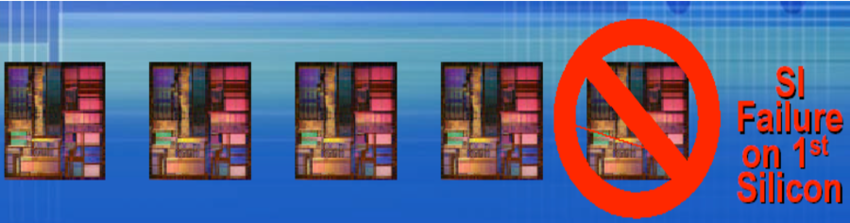
\includegraphics[width=1.0\textwidth]{Signal-Integrity-failures} \newline
	 
	 This is really a significant effect on the yield of the chip production
	\end{frame}

	%---------------------------------------------------------
	
	%-------------------------------------------
	
	\section{Crosstalk}
	
	\begin{frame}
		\frametitle{What is Crosstalk?}
	\begin{alertblock}
	
	Crosstalk is the transfer of a voltage transition from one switching net (aggressor) to another static or switching net (victim) through a coupling capacitance (Cc)
	
	\end{alertblock}
	\begin{center}
		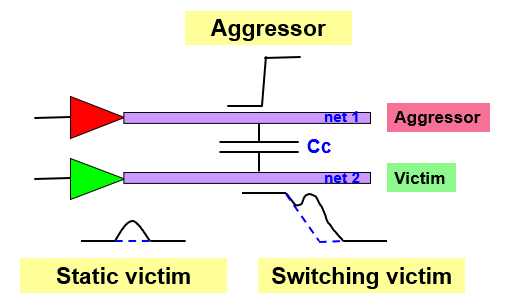
\includegraphics[width= 0.8\textwidth]{Crosstalk_wafe}
	\end{center}

	 
	\end{frame}
	%---------------------------------------------------------
	%Highlighting text
	\begin{frame}
		\frametitle{Crosstalk mechanism}
		Crosstalk is a very severe effect especially in \textcolor{red} { lower technology node }and high-speed circuits and it could be one of the main reason of \textcolor{red} {chip failure}.
		\newline
	
	\begin{alertblock}{Crosstalk mechanism}
		Crosstalk occurs via two mechanisms:
		\begin{itemize}
		\item Inductive Crosstalk
		\item Electrostatic crosstalk
		\end{itemize}
	\end{alertblock}
\end{frame}	
	%---------------------------------------------------
	\begin{frame}
		\frametitle{Inductive Crosstalk}
	\begin{itemize}
		\item Inductive crosstalk occurs due to \textcolor{red} {mutual inductance} between two nets.
		\item A varying current in a net creates a varying magnetic field around the net.
		\item A varying magnetic field can either radiate energy by launching radio frequency waves or it can couple to adjacent nets.
		\item Such coupling of the magnetic field is called \textcolor{red} {inductive crosstalk}. 
	\end{itemize}
		
	\end{frame}
	
	\begin{frame}
		\frametitle{Electrostatic crosstalk}
	\begin{itemize}
		\item Electrostatic crosstalk occurs due to mutual capacitance between two nets. 
		\item The electric voltage in a net creates an electric field around it. 
		\item If the electric field is changing, It can either radiate the Radio waves or can couple capacitively to the adjacent net. 
		\item Such coupling of the electric field is called \textcolor{red} {electrostatic crosstalk}
	\end{itemize}
		\begin{block}{Remark}
			Electrostatic Crosstalk mechanism is more significant and problematic than Inductive crosstalk. So, we will talk about Electrostatic crosstalk.
		\end{block}
	\end{frame}
	
	\begin{frame}
		\frametitle{Parasitic capacitances related to Interconnects}
		The main reason of crosstalk is the capacitance between the interconnects. \newline
		\begin{center}
				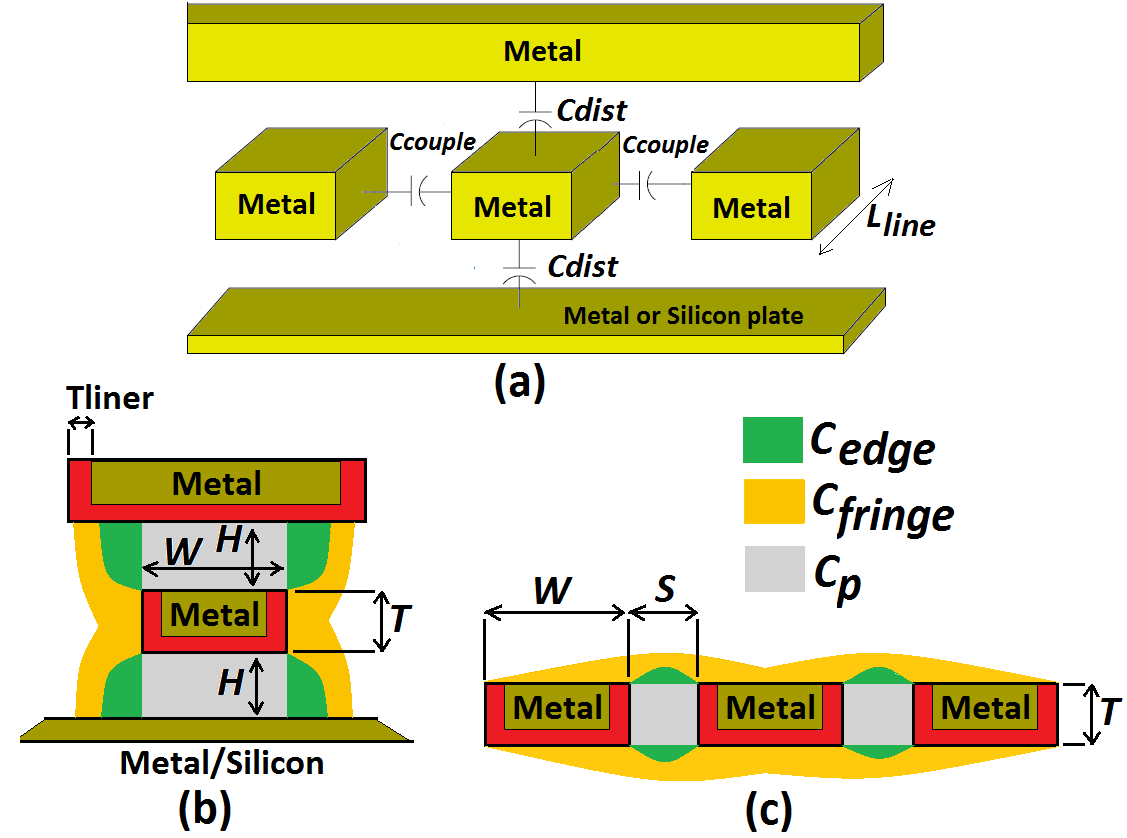
\includegraphics[width= 0.7\textwidth]{capacitance}
		\end{center}

	\end{frame}
	%-----------------------------------------------
	%--------------------------------------------------
	\section{Crosstalk Noise and Crosstalk Delay – Effects of Crosstalk}	
	\begin{frame}
		\frametitle{introduction}
	Crosstalk has two major effects
		\begin{block}
		
		\begin{itemize}
			\item Crosstalk glitch or crosstalk noise
			\item Crosstalk delta delay or crosstalk delay
		\end{itemize}
		\end{block}
		\begin{center}
		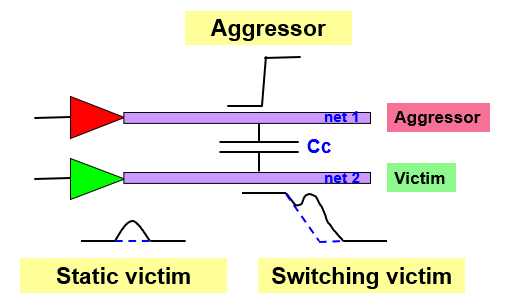
\includegraphics[width= 0.7\textwidth]{Crosstalk_wafe}
	\end{center}
	\end{frame}	
	
	\begin{frame}
		\frametitle{Crosstalk-Induced Noise (aka Glitches)}
			\begin{alertblock}
			
				Aggressor nets can create \textcolor{red} {crosstalk-induced noise} on static victim nets, also called “static noise”
				
			\end{alertblock}
		\begin{center}
			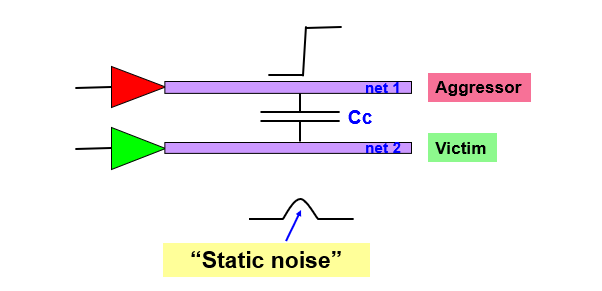
\includegraphics[width=0.9\textheight]{static_noise}
		\end{center}

	\end{frame}
	
	
	\begin{frame}
		\frametitle{Glitches types}
		Crosstalk glitch can be classified as below
	\begin{block}{Glitches types}
	\begin{itemize}
		\item Raising Glitch
		\item Failing Glitch
		\item Overshoot Glitch
		\item Undershoot Glitch
	\end{itemize}
\end{block}
\begin{itemize}
	\item \textbf{Rise glitch}: \textcolor{red}{Raising aggressor} net induces a rise glitch on a \textcolor{red}{steady low}
	\item \textbf{Fall glitch}: \textcolor{red}{Falling} aggressor net induces a fall glitch on a \textcolor{red}{steady high}
	\item\textbf{Overshoot glitch}: \textcolor{red}{Raising aggressor} net induces \textcolor{red}{overshoot glitch} on a \textcolor{red}{steady high} This takes the victim net voltage above its steady high value.
	\item \textbf{Undershoot glitch}: \textcolor{red}{Falling aggressor} net induces an \textcolor{red}{undershoot glitch} on a \textcolor{red}{steady low} This takes the victim net voltage below its steady low value.
\end{itemize}
	
	\end{frame}
	\begin{frame}
		\frametitle{Rise glitch}
		\begin{itemize}
			\item In this case, the aggressor net switches from logic 0 to logic 1 and the victim net is at constant zero as shown in the figure.
			\item As node A start switching from low to high, a potential difference across the mutual capacitance gets developed and the mutual capacitor Cm starts charging.
			\item During this event, there is some leakage current which starts flowing from node A to node V through the mutual capacitance Cm due to the leaky nature of mutual capacitance.
			\item This leakage current will raise the potential of node V, which creates a raising spike or raising glitch on the victim net as shown in figure.
		\end{itemize}
	\begin{center}
				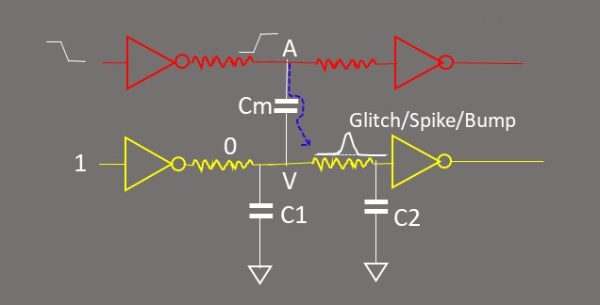
\includegraphics[width=0.5\textwidth]{crosstalk_noise1}
	\end{center}
\end{frame}
	\begin{frame}
	\frametitle{Fall glitch}
	\begin{itemize}
		\item In this case, the aggressor net switches from logic 1 to logic 0 and the victim net is at constant high as shown in the figure.
		\item As node A start switching from low to high, a potential difference across the mutual capacitance gets developed and the mutual capacitor Cm starts charging.
		\item During this event, there is some leakage current which starts flowing from node A to node V through the mutual capacitance Cm due to the leaky nature of mutual capacitance.
		\item This leakage current will drop the potential of node V, which creates a falling spike or falling glitch on the victim net as shown in figure
	\end{itemize}
	\begin{center}
		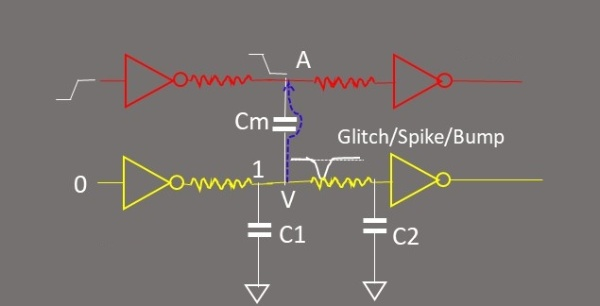
\includegraphics[width=0.5\textwidth]{fall_glitch}
	\end{center}
	\end{frame}	
%------------------------------------------
	\begin{frame}
		\frametitle{Effects of crosstalk glitch}
	\textcolor{red}{\textbf{Does every glitch unsafe?}}
	\newline
	The answer is it depends on the height of the glitch and the logical connection of the victim net. 
	\begin{itemize}
		\item If the height of the glitch is within the noise margin low (NML), Such a glitch is considered a safe glitch.
		\item If the glitch height is above the noise margin high (NMH), such a glitch is considered a potentially unsafe glitch. 
		\item In the case of a glitch, height is in between NMH and NML, this is an unpredictable case.
	\end{itemize}
			\begin{center}
			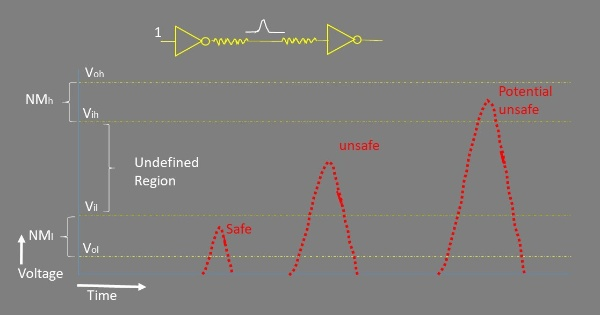
\includegraphics[width=0.5\textwidth]{safeandunsafeglitch}
		\end{center}
	\end{frame}	
%------------------------------------------
	\section{Crosstalk-Induced Delay}
	\begin{frame}
		\frametitle{Crosstalk-Induced Delay}
			\begin{alertblock}
				
			Aggressor/victim nets with overlapping timing windows can cause “crosstalk-induced delay” on victim nets. \newline
			This can lead to a speed-up or a slow-down of the victim net
		\end{alertblock}
	\begin{center}
		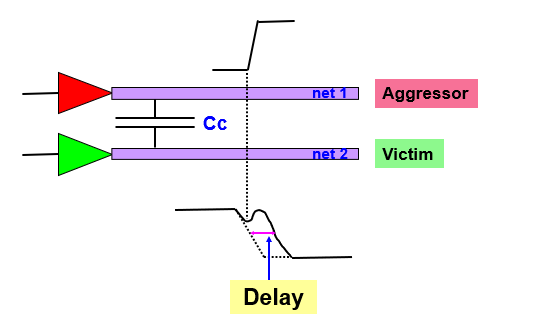
\includegraphics[width=0.7\textwidth]{delay}
	\end{center}
	\end{frame}	

\begin{frame}
	\frametitle{Crosstalk Delay}
	Crosstalk Delay can be classified as below
	\begin{block}{Crosstalk Delay types}
		\begin{itemize}
			\item Negative crosstalk delay
			\item Positive crosstalk delay
		\end{itemize}
	\end{block}
	\begin{block}{Notes}
	\begin{itemize}
		\item Crosstalk delay may cause setup and hold timing violation.
		\item Crosstalk could either increase or decrease the delay of a cell depending upon the switching direction of aggressor and victim nets.
	\end{itemize}
\end{block}
\end{frame}

%-----------------------------------------------
	\begin{frame}
	\frametitle{Positive crosstalk delay}
	\begin{itemize}
		\item Let’s consider aggressor net switches from low to high logic and victim net switches from high to low (opposite). as shown in figure.
		\item As node A starts to transition from low to high at the same time, node V starts switching from high to low.
		\item There is a coupling capacitance between A and V so the aggressor node will try to pull up the victim node.
		\item This will affect the smooth transition of the victim node from high to low and will have a bump after half of the transition and this will result in an increase in the transition time of the victim net.
	\end{itemize}
	\begin{center}
		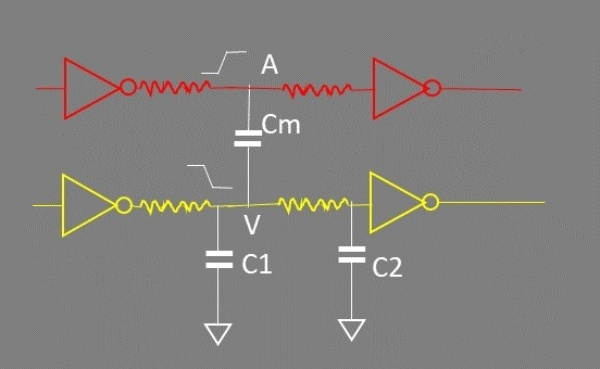
\includegraphics[width=0.45\textwidth]{crosstalkDelay1}
	\end{center}
\end{frame}

	\begin{frame}
	\frametitle{Negative crosstalk delay}
	\begin{itemize}
		\item Let’s consider the aggressor net switches from low to high logic and the victim net also switches from low to high (same direction). as shown in the figure.
		\item As node A starts to transition from low to high at the same time, node V also starts switching from low to high. 
		\item There is a coupling capacitance between A and V so the aggressor node will try to fast pull up the victim node. 
		\item This will affect the smooth transition of the victim node from low to high and will have a bump after half of the transition and this will result in a decrease in the transition time of the victim net. 
	\end{itemize}
	\begin{center}
		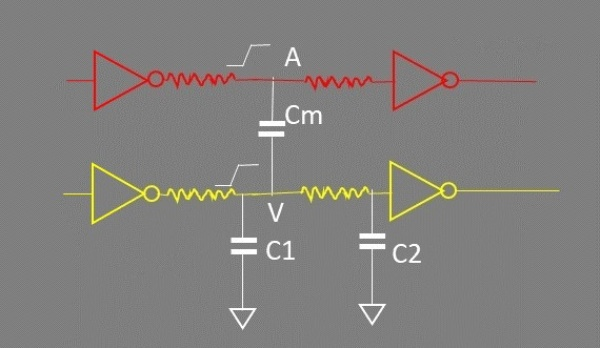
\includegraphics[width=0.45\textwidth]{crosstalkDelay2}
	\end{center}
\end{frame}
%-----------------------------------------------
\begin{frame}
	\frametitle{Effect on setup and hold timing}
	Crosstalk delay can violate the setup timing. Figure, shows the data path, launch clock path and capture clock path. 
	\begin{itemize}
		\item For setup timing, data should reach the capture flop before the required time of capture flop.
		\item if there is an increase of delay in the data path or launch clock path it may cause a setup violation.
		\item Setup violation may also happen if there is a decrease in delay on the capture clock path.  
	\end{itemize}
		\begin{center}
		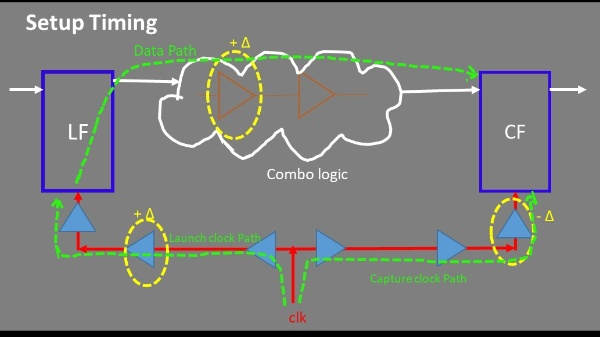
\includegraphics[width=0.45\textwidth]{setup}
	\end{center}
\end{frame}	

\begin{frame}
	\frametitle{Effect on setup and hold timing}
	Crosstalk delay can violate the hold timing. Figure, explains the situations where the hold time could violate due to crosstalk delay. 
	\begin{itemize}
		\item If there is a decrease in the delay of any cells in the data path and launch clock or there is an increase of delay of cells in the capture clock path due to crosstalk delay, It may result in the hold timing violation. ecrease in delay on the capture clock path.  
	\end{itemize}
	\begin{center}
		\includegraphics[width=0.6\textwidth]{hold}
	\end{center}
\end{frame}	
%------------------------------------------------

	\section{Crosstalk prevention techniques}	
	\begin{frame}
		\frametitle{prevention techniques}
	
	\begin{block}{Increase the spacing between aggressor and victim net}
		ncreasing the spacing between aggressor and victim net we are ultimately reducing the coupling capacitance between them as the capacitance is inversely proportional to the distance between them. So by increasing the spacing crosstalk will decrease.
	\end{block} 

			\begin{block}{Shielding of nets}
		By shielding a net the two things will happen, one is the direct coupling capacitance between the aggressor and victim net will vanish and secondly the shielding net will remain at a constant logic so there are no chances of crosstalk.
			\end{block} 
		
	\end{frame}
	\begin{frame}
		\frametitle{prevention techniques}
		\begin{block}{Upsizing the victim cell}
			If we increase the drive strength of the victim cell it will not be easy to affect by the aggressor net
		\end{block}
		
		\begin{block}{Downsize the aggressor cell}
			Higher the drive strength of aggressor cell, higher is the impact of crosstalk on the victim. So by reducing the drive strength we can reduce the crosstalk effect. 
		\end{block}
	\end{frame}
%--------------------------------------------------	
	\begin{frame}
		\frametitle{Wrap up}
		\begin{center}
			\<بِسْمِ اللَّـهِ الرَّحْمَـٰنِ الرَّحِيمِ> \\
			\<وَمَا أُوتِيتُمْ مِنَ الْعِلْمِ إِلَّا قَلِيلً>
			
		\end{center}
	\end{frame}	
\end{document}